%%%%%%%%%%%%%%%%%%%%%%%%%%%%%%%%%%%%%%%%%
% Masters/Doctoral Thesis 
% LaTeX Template
% Version 2.5 (27/8/17)
%
% This template was downloaded from:
% http://www.LaTeXTemplates.com
%
% Version 2.x major modifications by:
% Vel (vel@latextemplates.com)
%
% This template is based on a template by:
% Steve Gunn (http://users.ecs.soton.ac.uk/srg/softwaretools/document/templates/)
% Sunil Patel (http://www.sunilpatel.co.uk/thesis-template/)
%
% Template license:
% CC BY-NC-SA 3.0 (http://creativecommons.org/licenses/by-nc-sa/3.0/)
%
%%%%%%%%%%%%%%%%%%%%%%%%%%%%%%%%%%%%%%%%%

%----------------------------------------------------------------------------------------
%	PACKAGES AND OTHER DOCUMENT CONFIGURATIONS
%----------------------------------------------------------------------------------------

\documentclass[
10pt, % The default document font size, options: 10pt, 11pt, 12pt
%oneside, % Two side (alternating margins) for binding by default, uncomment to switch to one side
english, % ngerman for German
singlespacing, % Single line spacing, alternatives: onehalfspacing or doublespacing
%draft, % Uncomment to enable draft mode (no pictures, no links, overfull hboxes indicated)
%nolistspacing, % If the document is onehalfspacing or doublespacing, uncomment this to set spacing in lists to single
%liststotoc, % Uncomment to add the list of figures/tables/etc to the table of contents
%toctotoc, % Uncomment to add the main table of contents to the table of contents
%parskip, % Uncomment to add space between paragraphs
% nohyperref, % Uncomment to not load the hyperref package
headsepline, % Uncomment to get a line under the header
%chapterinoneline, % Uncomment to place the chapter title next to the number on one line
%consistentlayout, % Uncomment to change the layout of the declaration, abstract and acknowledgements pages to match the default layout
]{MastersDoctoralThesis} % The class file specifying the document structure

% \usepackage[hidelinks]{hyperref}

\usepackage[utf8]{inputenc} % Required for inputting international characters
\usepackage[T1]{fontenc} % Output font encoding for international characters

\usepackage{mathpazo} % Use the Palatino font by default

\usepackage[backend=bibtex,style=ieee]{biblatex} % Use the bibtex backend with the authoryear citation style (which resembles APA)

% \usepackage[block=ragged,natbib=true]{biblatex}

\usepackage{subcaption} % for subfigures

\usepackage{tikz}
\usetikzlibrary{positioning,arrows,fit,backgrounds, patterns}

\usepackage[super]{nth}

\addbibresource{references.bib} % The filename of the bibliography

\usepackage[autostyle=true]{csquotes} % Required to generate language-dependent quotes in the bibliography

\usepackage{layout}

\usepackage{graphicx}

%----------------------------------------------------------------------------------------
%	TOC SETTINGS
%----------------------------------------------------------------------------------------

\setcounter{secnumdepth}{2} % only chapter and sections and subsections will be numbered
\setcounter{tocdepth}{2}    % entries down to \subsections in the TOC

%----------------------------------------------------------------------------------------
%	MARGIN SETTINGS
%----------------------------------------------------------------------------------------

\geometry{
	paper=a4paper, % Change to letterpaper for US letter
	inner=2.5cm, % Inner margin
	outer=3.8cm, % Outer margin
	bindingoffset=.5cm, % Binding offset
	top=1.5cm, % Top margin
	bottom=1.5cm, % Bottom margin
	%showframe, % Uncomment to show how the type block is set on the page
}

\hyphenation{Mou-gia-ka-kou}

%----------------------------------------------------------------------------------------
%	THESIS INFORMATION
%----------------------------------------------------------------------------------------

\thesistitle{Title of thesis} % Your thesis title, this is used in the title and abstract, print it elsewhere with \ttitle
\supervisor{Prof. Dr. \textsc{Surname} FirstName} % Your supervisor's name, this is used in the title page, print it elsewhere with \supname
\coadvisor{Prof. Dr. \textsc{Surname} FirstName} % Your examiner's name, this is not currently used anywhere in the template, print it elsewhere with \examname
\degree{Doctor of Philosophy in XXX} % Your degree name, this is used in the title page and abstract, print it elsewhere with \degreename
\author{\textsc{Surname} FirstName} % Your name, this is used in the title page and abstract, print it elsewhere with \authorname

\matriculation{00-000-000} % Your matriculation number, this is not currently used anywhere in the template, print it elsewhere with \matriculationnum

\subject{SUBJECT} % Your subject area, this is not currently used anywhere in the template, print it elsewhere with \\subjectname
\keywords{keyword1, keyword2} % Keywords for your thesis, this is not currently used anywhere in the template, print it elsewhere with \keywordnames
\university{University of Bern} % Your university's name and URL, this is used in the title page and abstract, print it elsewhere with \univname
\department{Faculty of XXX} % Your department's name and URL, this is used in the title page and abstract, print it elsewhere with \deptname
\group{Group Name} % Your research group's name and URL, this is used in the title page, print it elsewhere with \groupname
\faculty{Graduate School for Cellular and Biomedical Sciences} % Your faculty's name and URL, this is used in the title page and abstract, print it elsewhere with \facname

\newcommand*{\resetfigpath}[1]{
    \graphicspath{{chapters/#1/pics/}}
}

\graphicspath{{pics/}}

\begin{document}

\frontmatter % Use roman page numbering style (i, ii, iii, iv...) for the pre-content pages

\pagestyle{plain} % Default to the plain heading style until the thesis style is called for the body content

%----------------------------------------------------------------------------------------
%	TITLE PAGE 1
%----------------------------------------------------------------------------------------

\begin{titlepage}

\hfill{
\includegraphics[width=4.5cm]{Logo-unibe}}

\begin{center}

\vspace*{0.5cm}
{\Large \facname \\ \textsc{\univname} \par}\vspace{1cm} % University name

{\huge \bfseries \ttitle\par}\vspace{1cm} % Thesis title
\large{PhD Thesis submitted by}\vspace{0.5cm}

{\Large \bfseries \authorname \par}\vspace{0.5cm}

\large{from }{\Large \bfseries Place of Origin \& Canton \par}\vspace{0.5cm}

\large{from }{\Large \bfseries Country of Origin \par}\vspace{0.5cm}

\large{for the degree of XXX}\vspace{0.5cm}
 
\vfill

\large{Supervisor \\ \supname \\ Supervisor Institute/Department of YYY}\vspace{0.5cm}

\large{Co-advisor \\ \examname \\  Co-advisor Institute/Department of YYY}\vspace{0.5cm}

% % this is needed for the publication at the university of bern library
% \footnotesize{Original document saved on the web server of the University Library of Bern\\}
% 
\includegraphics[width=1.5cm]{cc88x31}\\
% \footnotesize{This work is licensed under a \href{https://creativecommons.org/licenses/by-nc-nd/2.5/ch/}{Creative Commons Attribution-NonCommercial-NoDerivs 2.5 Switzerland License}.}
\end{center}
\end{titlepage}
\cleardoublepage

% %----------------------------------------------------------------------------------------
% %	TITLE PAGES 2
% %----------------------------------------------------------------------------------------
% {
% \pagenumbering{gobble}
% \vspace*{5cm}
% \begin{center}
% \textbf{\Large{Copyright Notice}}
% \end{center}

% \noindent This document is licensed under the Creative Commons Attribution-Non-Commercial-No derivative works 2.5 Switzerland. 
% \url{http://creativecommons.org/licenses/by-nc-nd/2.5/ch/} \\

% \noindent\textbf{\large{You are free:}}\\
% \noindent\textbf{Share.} copy and redistribute the material in any medium or format. \\

% \noindent\textbf{\large{Under the following conditions:}}\\
% \textbf{Attribution.} You must give appropriate credit, provide a link to the license, and indicate if changes were made. You may do so in any reasonable manner, but not in any way that suggests the licensor endorses you or your use.  \\
% \textbf{Non-Commercial.} You may not use the material for commercial purposes.  \\
% \textbf{No derivative works.} If you remix, transform, or build upon the material, you may not distribute the modified material.  \\

% \noindent For any reuse or distribution, you must make clear to others the license terms of this work.  \\

% \noindent Any of these conditions can be waived if you get permission from the copyright holder. \\

% \noindent Nothing in this license impairs or restricts the author’s moral rights according to Swiss law. \\

% \noindent The detailed license agreement can be found at: \url{http://creativecommons.org/licenses/by-nc-nd/2.5/ch/legalcode.de}
% \cleardoublepage
% \pagenumbering{roman}
% % \clearpage

%----------------------------------------------------------------------------------------
%	TITLE PAGES 3
%----------------------------------------------------------------------------------------

\cleardoublepage

%----------------------------------------------------------------------------------------
%	TITLE PAGES 4
%----------------------------------------------------------------------------------------

\vspace*{\fill}

\noindent Accepted by the Faculty of Medicine, the Faculty of Science and the Vetsuisse Faculty of the University of Bern at the request of the Graduate School for Cellular and Biomedical Sciences

\vspace{3cm}

\noindent Bern, 	Dean of the Faculty of Medicine

\vspace{3cm}

\noindent Bern, 	Dean of the Faculty of Science

\vspace{3cm}

\noindent Bern, 	Dean of the Vetsuisse Faculty Bern

\vspace{3cm}

\vspace*{\fill}

\cleardoublepage

%----------------------------------------------------------------------------------------
%	ABSTRACT PAGE
%----------------------------------------------------------------------------------------

\begin{abstract}
\addchaptertocentry{\abstractname} % Add the abstract to the table of contents
Lorem ipsum dolor sit amet, consectetur adipiscing elit. Nam bibendum, mi non lacinia aliquet, orci nisi commodo ex, ac malesuada nunc libero eget metus. Proin vel enim risus. Nullam lobortis posuere sodales. Quisque ac placerat sapien. Praesent in pulvinar dolor. Pellentesque faucibus quam at dui consectetur scelerisque. Donec laoreet pharetra neque, id cursus metus venenatis eu. Quisque tempor molestie velit, ac euismod ligula ullamcorper a. Aliquam lacus ligula, ultrices id vehicula et, hendrerit non turpis. Phasellus molestie erat quis sem iaculis, sed posuere metus tempus. Nullam suscipit lorem et accumsan convallis. Cras eleifend mauris ultrices nunc hendrerit condimentum. 
\\
\textbf{Keywords --} \keywordnames
\\ ~ \\ ~ \\ ~ \\
\end{abstract}

%----------------------------------------------------------------------------------------
%	ACKNOWLEDGEMENTS
%----------------------------------------------------------------------------------------

\begin{acknowledgements}
\addchaptertocentry{\acknowledgementname} % Add the acknowledgements to the table of contents
Lorem ipsum dolor sit amet, consectetur adipiscing elit. Nam bibendum, mi non lacinia aliquet, orci nisi commodo ex, ac malesuada nunc libero eget metus. Proin vel enim risus. Nullam lobortis posuere sodales. Quisque ac placerat sapien. Praesent in pulvinar dolor. Pellentesque faucibus quam at dui consectetur scelerisque. Donec laoreet pharetra neque, id cursus metus venenatis eu. Quisque tempor molestie velit, ac euismod ligula ullamcorper a. Aliquam lacus ligula, ultrices id vehicula et, hendrerit non turpis. Phasellus molestie erat quis sem iaculis, sed posuere metus tempus. Nullam suscipit lorem et accumsan convallis. Cras eleifend mauris ultrices nunc hendrerit condimentum. 
\end{acknowledgements}

%----------------------------------------------------------------------------------------
%	LIST OF CONTENTS/FIGURES/TABLES PAGES
%----------------------------------------------------------------------------------------

\tableofcontents % Prints the main table of contents

% \listoffigures % Prints the list of figures

% \listoftables % Prints the list of tables

%----------------------------------------------------------------------------------------
%	ABBREVIATIONS
%----------------------------------------------------------------------------------------

\begin{abbreviations}{ll} % Include a list of abbreviations (a table of two columns)
\end{abbreviations}

%----------------------------------------------------------------------------------------
%	DEDICATION
%----------------------------------------------------------------------------------------

\dedicatory{Dedication}

%----------------------------------------------------------------------------------------
%	THESIS CONTENT - CHAPTERS
%----------------------------------------------------------------------------------------

\mainmatter % Begin numeric (1,2,3...) page numbering

\pagestyle{thesis} % Return the page headers back to the "thesis" style

% Include the chapters of the thesis as separate files from the Chapters folder
% Uncomment the lines as you write the chapters

\resetfigpath{1-intro}

\chapter{Introduction}
\label{intro}

The medical imaging field has recently witnessed the revolution of \gls{ai}, a broad discipline that is a part of computer science whose aim is to conceptualize human ``intellectual'' tasks, and produce computer programs that can replicate them, thereby allowing to relieve human beings from tedious and repetitive tasks.
From classification to segmentation tasks, \gls{ai} already provides flexible and efficient tools that greatly facilitate the daily practice of clinicians.
In particular, large quantities of \gls{mri} brain scans are now efficiently and accurately processed by \gls{ai} systems that help clinicians in the diagnosis of pathologies \cite{sun19}.
Similarly, surgical instruments can be segmented automatically and accurately in real-time to allow laparoscopic interventions of the abdominal cavity by means of robotic technology, thereby decreasing the invasiveness of traditional methods \cite{davinci}.

\Gls{ml}, a term that denote a sub-category of \gls{ai}, is grounded on the ``learning by example'' paradigm.
Whereas traditional approaches generally consisted in explicitly formalizing and implementing complex tasks as a combination of simpler programmatic instructions,
\gls{ml} rather considers that a flexible system can learn such instructions automatically through repeated experiences.

Concretely, as a young child can effectively derive the concept of car using a few visual examples, and be able to identify an ``unseen'' car in a complex environment with near-perfect accuracy,
state-of-the-art \gls{ml} methods leverage the same principle.
However, no matter how well-engineered they are, they need, in order to replicate this simple task with comparable accuracy, thousands of examples and counter-examples of images \cite{ILSVRC15}.

In this scenario, collecting such quantity of example images and annotating them is tedious and cumbersome.
In practice, the annotation task is performed by numerous individuals in parallel.
The annotation of medical data, however, adds the following practical difficulties.
First, the task can require a specific medical expertise.
Second, assuming such experts are available and willing to participate to this task, their daily obligations imposes a limited time budget.
These two factors largely explain why the medical field does not benefit from the latest and greatest \gls{ml} technologies used in more generic applications \cite{orting19}.


\section{Proposed annotation protocol and applicability}

In the present thesis, we devise solutions that allow to annotate medical sequences in a fast and intuitive manner, in an attempt to alleviate the bottleneck of scarcity of example data.

In particular, the annotator is presented a video or volumetric sequence that plays on a screen, i.e. the frames unfold in an automatic manner.
As the sequence unfolds, the annotator is asked to point at the object of interest using a pointing device, such as a mouse, a tablet pen, or an eye-gaze tracker.
In contrast with the traditional approach, where the object must be manually segmented on each frame individually, the proposed protocol drastically reduces the annotation time.
In essence, our contribution ambitions an annotation time equal to the duration of the video/volume playback.
For example, assuming the sequence contains $100$ frames playing at $5fps$, the total annotation time is $20$ seconds.
In comparison, the traditional pixel-wise annotation task of a sequence of similar size could take anywhere from $10$ min. to $1$ hour.

Concretely, we set the following requirements on the annotation protocol:
\begin{itemize}
  \item The annotator does not need to manually change the frame being annotated, e.g. by hitting a forward or backward key. The sequence automatically unfolds according to a specified frame-rate.
  \item The annotator handles a single pointing device, which he/she uses to indicate the location of the object of interest.
  \item The annotator must be able to watch and annotate the sequence in a single go, i.e. he/she does not need to review annotations and modify them manually afterwards.
\end{itemize}

The segmentation method must be functional in a variety of situations, namely produce acceptable accuracy for:
\begin{itemize}
  \item Both videos and volumetric sequences.
  \item Both color and grayscale images.
  \item Various kind of image modality, e.g. \gls{mri} and \gls{ct}.
  \item Various levels of noise, perturbations, and lightning artifacts.
  \item Various nature of object, i.e. size, shape, appearance.
  \item The object can be made of several parts that are not immediately contiguous, i.e. an \gls{mri} brain scan with several tumors.
\end{itemize}

\section{Datasets}

We now introduce the datasets that have been used during the elaboration and testing of the proposed solutions.
Note that as the range of possibilities is huged, we chose to restrict ourselves to $4$ types of sequences. These, however, cover the entirety of the proposed spectrum.

In particular, we now describe them in detail and give each type a short name that will be used in the remaining of this thesis:

\begin{itemize}
  \item \textbf{Tweezer}: Surgical instruments during an endoscopic procedure, where the instrument is object of interest.
    The background is relatively homogeneous, while the instrument moves accross the frame both in translation and rotation.
    The sequences are taken from the MICCAI EndoVision Challenge \cite{EndoChall}.
    Each sequence is around $120$ frames long, i.e. represent $\sim 5s$ of video acquired at $25$ fps.
  \item \textbf{Cochlea}: Volumetric \Gls{ct} scans of the inner-ear where the cochlear labyrinth is to be segmented. These are acquired according to different protocols, and therefore show important variations in gray-scale level, orientation, as well as sizes. Furthermore, the object of interest is composed of different parts that split and merge.
  \item \textbf{Slitlamp}: Microscopic video of the retina where the optic nerve is to be segmented. The videos have been acquired using a slitlamp instrument.
    The optic nerve is of rather small size. The background often shows important artifacts, in the form of yellow and blue beams, which sometime overlap with the object of interest. The movement of the optic nerve is often very jerky.
  \item \textbf{Brain}: Transverse \gls{mri} scans of brains where the tumor is object of interest. The sequences are taken randomly from the Brain Tumor Segmentation Challenge (BRATS) public database \cite{BRATSChall}.
    Scans are acquired using the same \gls{mri} protocol, but with different scanners, thereby showing wide variety of contrast and color.
    The tumors have varying size, colors, and shapes. Sometimes, the same scan shows several tumors on the same slice.

\end{itemize}

In Fig. \ref{fig:dset_previews}, we show example frames for each type.

\begin{figure}
\centering
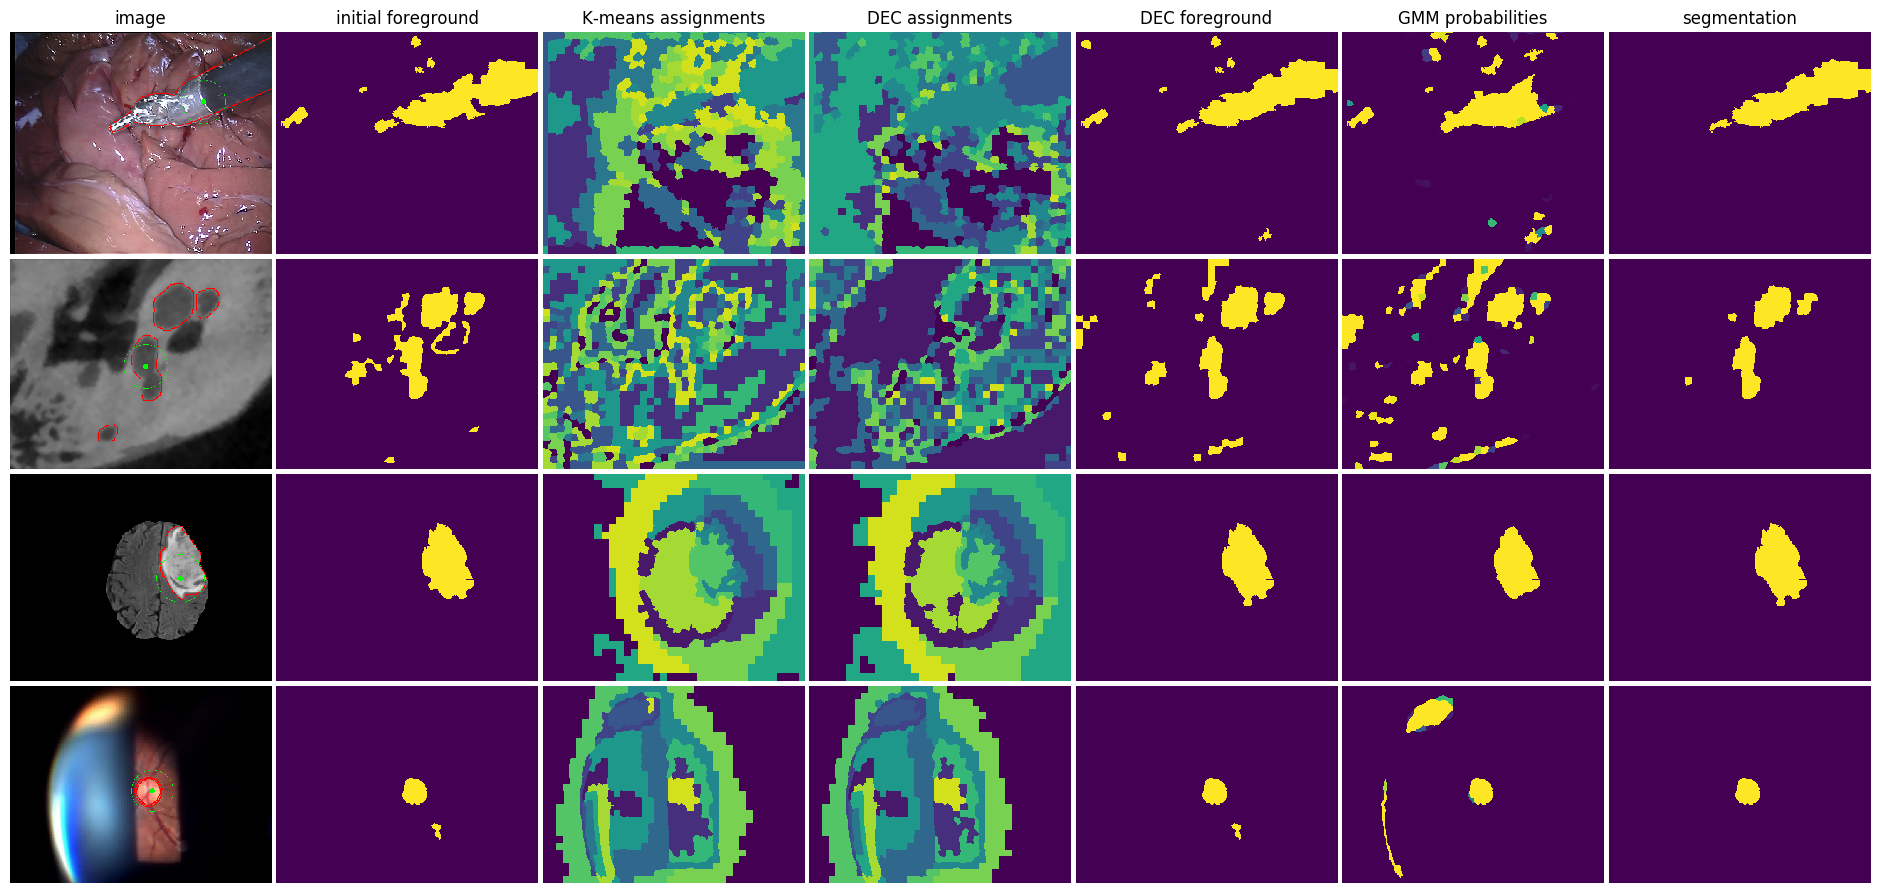
\includegraphics[width=0.99\textwidth]{prevs.png}
\caption{Example of objects of interest in different video and volumetric modalities. Each type contains 4 sequences. We show a single frame per sequence.
  From top to bottom: Tweezer, Cochlea, Slitlamp, and Brain}
\label{fig:dset_previews}
\end{figure}

\section{Annotation Software and Web Platform}
In the frame of this thesis, a flexible and elegant annotation software was developed that supports as pointing device a traditional mouse, a pen compatible with touch-screens, as well as an interface to connect a eye-gaze tracker through the USB port.
Also, a web interface was designed and implemented that allows a user to upload a sequence annotated using the above software, and download the generated pixel-wise segmentation when they are ready.
We now describe both contributions.

\subsection{Sequence annotation tool}
\label{sec:anna}

The typical annotation workflow is as follows:

\begin{enumerate}
  \item[-]{Provide as input a volume/video. These can be either DICOM \cite{dicom}, or video files.}
  \item[-]{Optional: Set the framerate at which the sequence will play (right knob on Fig. \ref{fig:anna}).}
  \item[-]{Optional: Connect the software to the eye-gaze tracker server. The tracker will then act as a secondary mouse.}
  \item[-]{Hit the play button. The sequence unfolds.}
  \item[-]{Give point annotations:}
    \begin{itemize}
      \item[-]{When using mouse: Simply click on the desired region.}
      \item[-]{When using gaze-tracker: Place gaze on region and use right button (Fig. \ref{fig:anna}) to activate the recording of locations.}
    \end{itemize}
  \item[-]{Save locations in \gls{csv} file.}
\end{enumerate}

\begin{figure}[!htpb]
  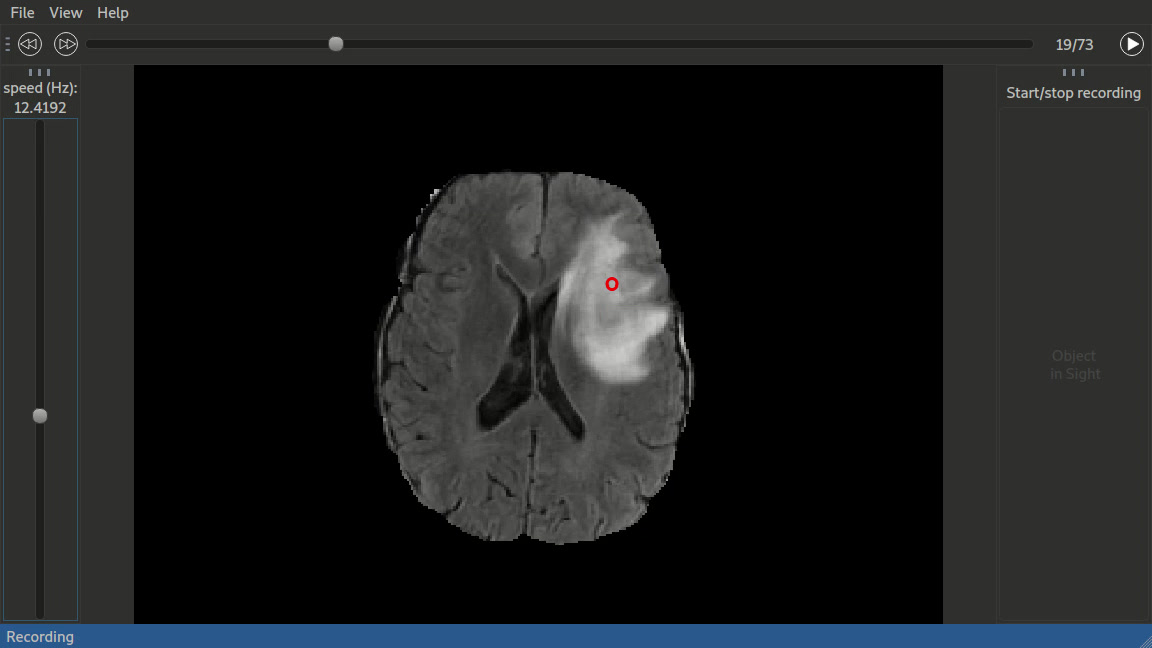
\includegraphics[width=0.99\textwidth]{anna0.png}
  \caption{Screenshot of annotation tool. }
  \label{fig:anna}
\end{figure}

The software is intended to be cross-platform and be compatible with a variety of input formats.
Second, as our early experiments relied on an eye-gaze tracker, our software needed to be compatible with the proprietary backend given by the manufacturer.
Third, a simple \gls{gui} was needed to display images and allow the user to select his favorite modality of annotation.
The latter requirements drove our choice towards the Qt5 framework \cite{eng16}, which relies on C++ and provides convenient widgets out of the box.
Our software supports allows to annotate using a mouse and an eye-gaze tracker \cite{eyetribe}.
As platform, it supports the Linux, MacOS and Windows operating systems.
We provide the source code at \href{https://github.com/aimi-lab/Anna}.

\subsection{Web platform}
The segmentation methods presented in the next chapters require important computational resources, namely a \gls{gpu} to train deep networks.
We therefore provide a way for users to upload their data along with the corresponding 2D locations to a server that will perform the necessary computations remotely and send back segmentation results when they are available.
Concretely, we develop a web interface that provides:

\begin{itemize}
  \item[-]{Links to download the annotation software (Sec. \ref{sec:anna}).}
  \item[-]{A login mechanism that provides us with a contact e-mail address.}
  \item[-]{An upload form where the user drops his sequence along with the 2D locations}
\end{itemize}

Once the data has been uploaded, a task object is created and queued until computational resources are available.
After completion, the user is warned that he can download his segmentations via a URL.

\begin{figure}[!htpb]
  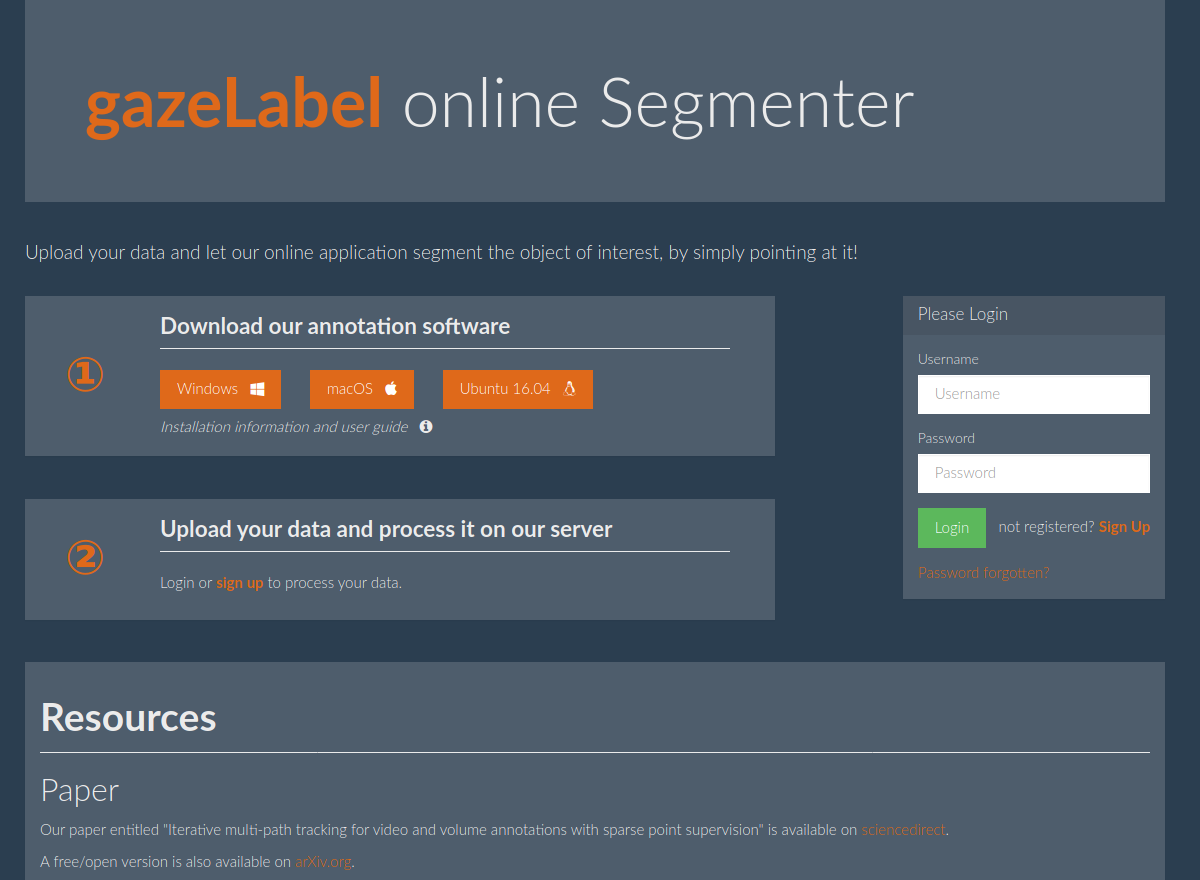
\includegraphics[width=0.99\textwidth]{gazelabel.png}
  \caption{Screenshot of our web platform. Home page.}
  \label{fig:anna}
\end{figure}

The frontend, which generates the web pages uses the \href{https://webpack.js.org}{Webpack} bundler.
The backend is based on the \href{https://www.djangoproject.com/}{Django} framework, which handles different applications, namely the forms (login, data upload), the job queue, and the database.

\begin{figure}[!htpb]
  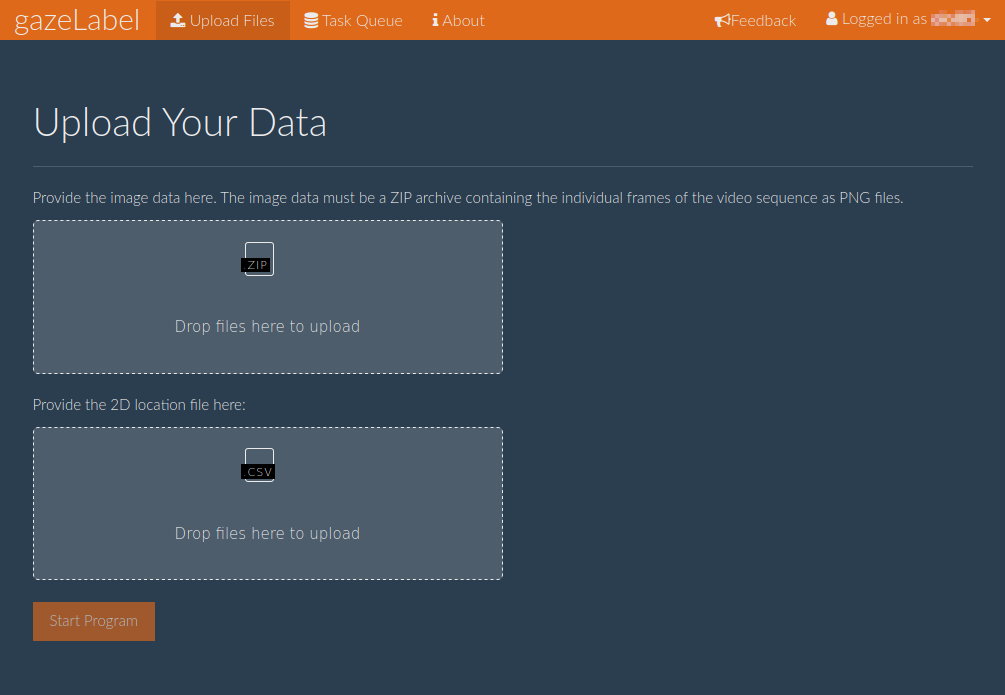
\includegraphics[width=0.99\textwidth]{gazelabel_upload.png}
  \caption{Screenshot of our web platform, where the user can upload a sequence and its corresponding annotations. The task queue panel shows the state of the submitted tasks.}
  \label{fig:anna_upload}
\end{figure}



\section{Related Works}

Past research that address this issue can be roughly divided in two categories,
where the first leverages computer vision techniques to generate segmentation masks from sparse and/or noisy annotations, while the second focuses on developping Machine Learning techniques to minimize an annotation budget.
In practice, both categories often overlap.

We start by giving an overview of state-of-the-art in computer vision.
Next, we focus on \gls{ml} methods.
In particular, we emphasize on domains that target segmentation in a semi-supervised setting.

\subsection{Computer Vision Methods}
Another line of research focuses on the annotation protocol itself so as to complement the above efforts.
While the most tedious protocol requires that images be manually segmented at a pixel-level, many computer-vision approaches exist to facilitate this task.

Early contributions relied on the Active Contour model \cite{kass88}, which assumes that an initial contour is given and parameterized as the nodes of a spline curve, in this context called an elastic snake.
The segmentation problem is formulated as finding the deformation of the initial snake that minimizes an energy term.
In its simplest form, the energy term is composed of a term that determines the fitting of the snake to the edges of the image, while another term controls the smoothness of the snake.
The energy is then minimized using gradient descent.
Following works alleviate the problem of robustness brought by noisy edge maps by minimizing the Mumford-Shah functional \cite{chan01}, and parameterize the contour using the level-set method \cite{osher88}.

More recently, annotations in the form of scribbles were considered, where the annotator is asked to draw crude delineations of one or several objects of interest, along with a scribble on the background.
A first method that handles such kind of annotations relies on the Random-Walk algorithm \cite{grady06}.
The segmentation problem reduces to assigning to each unlabeled pixel a random-walker. The label of the latter pixel is then determined by the finding the label for which the walker has a maximum probability of reaching first.

Relying on the same annotation requirement, the graph-cut approach \cite{Boykov2006}
minimizes an Markov Random Field energy objective that considers unary terms (a scalar on each pixel), and a pairwise term that models the similarity of neighboring pixels.
Concretely, the image or volume is represented as a region adjacency graph where each pixel is assigned a node, and edges connect adjacent pixels.
Each annotated positive pixels is connected to a source node, while annotated negatives are connected to a sink node.
The energy minimization is then performed using the min-cut/max-flow algorithm \cite{goldberg88}.
Using the same algorithm, grab-cut \cite{rother04}, further simplifies the scribble-based annotation protocol by considering bounding-boxes around the object of interest, which provide crude labels on both foreground and background in a single stroke.

Along the same line, \cite{criminisi08}

\subsection{On the Wise Use of Annotation Budget}
The problem of scarcity of labeled data can also be posed in the following manner:
Given a limited annotation budget, i.e. when only a few hours of annotation work can be provided, how can one make the best use of it?

\gls{al} \cite{settles09} considers semi-supervised learning scenarios, where abundant unlabeled data are available.
\gls{al} algorithms select unlabeled samples that are the most informative to the \gls{ml} model, i.e. it assumes that many unlabeled samples represent redundant information to the late-stage \gls{ml} model.
In \cite{KonSznFua15}, authors devise a strategy to select unlabeled supervoxels of a 3D volume so as to segment volumes of various modalities.
The approach iteratively trains a classifier and takes its entropy as measure of uncertainty.
Combining the latter with a geometric prior, which takes into account intuitive rules on spatial coherence, they sample a batch of most uncertain samples.
The classifier is then re-trained using the newly annotated samples.

Crowd-sourcing, refers to the outsourcing of the annotation task to a high number of annotators \cite{orting19}.
Its use in the frame of medical imaging poses several limitations.
First, the difficulty of the annotation task can prohibit the effective use of crowd-sourcing, e.g when the structure of interest is hard to distinguish \cite{orting19}.
Another limitation is the nature of the data, i.e. one usually prefers to pre-classify brain scans and submit to workers the slices where tumors are present.
Last, one must usually integrate a test-task to ensure the competence of workers, or filter-out annotations provided by ``poorly performing'' workers \cite{park18}.

\subsection{Transfer Learning, Semi-supervised Learning, and Domain Adaptation}
\gls{tl} consists in using a \gls{ml} model trained for the task of interest, but using a training set of different nature than the targeted domain, e.g. train a \gls{cnn} to segment natural objects (trees, cars, ...) for the segmentation of surgical tools.
As pointed out by \cite{oliver18}, an important and implicit assumption in that context is that both datasets share similar data distributions.

\gls{ssl} is a broad category of \gls{ml} algorithm that combines traditional supervised learning tasks, where a fully labeled training dataset is available, along with an abundant unlabeled dataset.
The latter can, under specific conditions, boost the performance of an \gls{ml} model trained with labeled dataset only, i.e. in a fully-supervised manner.
The basic idea is that the ML model may acquire knowledge of the data distribution from the unlabeled set.
Here again, one assumes that both data domains share similar distributions.
In \cite{ghafoorian17}, authors show experimentally that a \gls{nn} trained to segment tumors on MRI brain scans acquired in a given MRI protocol, perform poorly when transfered to another protocol, as the shape, intensities, and contrast level are inconsistent.

\gls{da} addresses the problem of adapting the model so as to take into account domain shift, i.e. the discrepancies between the training and target domain.
In \cite{perone19}, authors devise a strategy to segment MRI scans of spinal cords using a model trained with images taken at a specific field-of-view, and transfer to another field-of-view in an unsupervised fashion.
Their approach leverages data-augmentation to enforce a consistency between the augmented and pristine images of the unlabeled set, while jointly training with the labeled set with traditional cross-entropy loss.
On the same image modality, \cite{li20} resort to adversarial training. They jointly train a segmentation model and a discriminator wit shared weights. The discriminator is trained to discriminate between the source and target domain.





%%% Local Variables:
%%% mode: latex
%%% TeX-master: "../../main"
%%% End:

\resetfigpath{2-eel}

\chapter{Expected exponential loss for gaze-based video and volume}
\label{eel} % For referencing the chapter elsewhere, use \ref{Chapter1}

\section{Notation}
Let an image sequence (or volume) be denoted $\mathcal{I} = [I_{0}, \cdots , I_{T}]$ and let $\mathcal{G} = \{g_{t} \}^{T}_{t=0}$ such that $g_t\in \mathbb{R}^{2}$ is a 2D gaze pixel location in $I_{t}$.

While we ideally would like
a pixel-wise segmentation, we choose to decompose each image using a temporal superpixel
strategy \cite{chang13} and operate at a superpixel level instead.

We thus let $I_t$ be described by the set of non-overlapping superpixels
$S_{t} = \{S^{n}_t\}^{N_t}_{n=0}$ and define the set of all superpixels across all
images as $\mathcal{S} = \{S_t \}^{T}_{t=0}$.
We denote the set $\mathcal{P} = \{S^{n}_t | g_{t} \subset S^{n}_t, t = 0, \cdots, T, n = 0, \cdots, N_t \}$ as all
superpixels observed and the rest as $\mathcal{U} = \mathcal{S} \backslash \mathcal{P}$.
We associate with each $S^{n}_t$ a binary random variable $Y^{n}_{t} \in \{-1, 1\} = \mathcal{Y}$,
such that $Y^{n}_t = 1$ if $S^{n}_t$ is part of the object and -1 otherwise.
In particular, we defined $Y_n$ as a Bernoulli random variable, $Y^{n}_t \sim Ber(\epsilon_{S^{n}_{t}})$, $\epsilon \in (0,1)$.
Note that for positive superpixels $S^{n}_t \in \mathcal{P}$, we consider these as part of the object and let $Y^{n}_t = 1$ with $\epsilon_{S^{n}_{t}}=1$.

\section{Method}
Our goal is to train a prediction function, $f : S \rightarrow Y$
that takes into account observed superpixels as well as the unobserved ones.
To do this we propose the following Expected Exponential Loss (EEL) function:

\begin{equation}
  \mathcal{L}_{EEL} = \mathbb{E}^{Y} \left[ \sum_{S \in \{ \mathcal{P}, \mathcal{U}\}} e^{-f(S)Y}\right]
\end{equation}

where the expectation is taken with respect to all $Y$s.
By linearity of expectation and the fact that labeled superpixels have no uncertainty in their label, we can rewrite the loss for all superpixels as

\begin{equation}
  \label{eq:eel}
  \mathcal{L}_{EEL} = \sum_{S \in \mathcal{P}} e^{-f(S)} + \left( \sum_{S \in \{ \mathcal{P}} \epsilon_{S} e^{-f(S)Y} + (1-\epsilon_{S}) e^{f(S)Y}\right)
\end{equation}

Note that Eq. \ref{eq:eel} is a generalization of the Exponential Loss (EL) \cite{hastie09}.
In the case where labels are known, the loss is the same as the traditional loss as the expectation is superfluous.
For unknown samples, the value of $\epsilon_{S}$ weighs the impact of the superpixels.
For instance, if $\epsilon_{S}$ is close to 0.5, the sample does not affect the loss.
Conversely values of $\epsilon_{S}$ close to 1 (or 0) will strongly impact the loss.

\section{Implementation}
We implemented the above EEL within a traditional Gradient Boosting classifier \cite{hastie09},
by regressing to the residual given by the derivate of Eq. \ref{eq:eel}.
For all experiments, we used stumps as weak learners, a shrinkage factor of 1 and the line search was replaced by a constant weight of 1.
The weak learner stumps operate on features extracted from the center of the superpixel.
In particular, we used generic Overfeat features \cite{sermanet13} which provide a rich
characterization of a region and its context (e.g. 4086 sized feature vector).
During training we used all superpixels in $\mathcal{P}$ and used $10\%$ of those in U.
A total of 50 boosting rounds was performed in all cases.
To predict segmentations for the entire volume, we
predicted the remaining $90\%$ of superpixels in $\mathcal{U}$.

\section{Probability estimation for unknown labels}
\label{sec:eel_estim}
To estimate $\epsilon_{S}$ in Eq. \ref{eq:eel}, we take inspiration from the Label Propagation method \cite{zhou04}, which uses a limited number of positive and negative samples to iteratively propagate labels to unobserved samples.
In our setting however, we only propagate positive samples to unlabeled
samples using the gaze information as well as pixel motion estimation to constrain the probability diffusion.
We let $P_{0} = \left[p_0,\cdots, p_{N}\right]$ be a vector of initial probabilities for all superpixels in a given image, where $p_n = P(Y = 1|\mathcal{P})$ is the probability that superpixel $S_{n}$ is part of the object.
In practice, we estimate $p_{n}$ by computing a gaze dependent Lab color model using all gaze
locations and assessing how likely a superpixel $S_{n}$ is part of the object.
That is, we compute

\begin{equation}
  p_{n} = \max_{S \in \mathcal{P}} \mathcal{N}(S_{n}|\mu_{s},\Sigma_{S})
  \end{equation}

  where $\mathcal{N}$ is a Gaussian distribution such that $\mu_{S}$ and $\Sigma_{S}$ are the color mean and covariance of pixels in a positive superpixel $S$.
  Also, we fix $p_{n}=1$ for positive superpixels.
  To propagate probabilities, we also define a $N \times N$ affinity matrix, denoted W
with values

\begin{equation}
w_{ij} = exp(-||\theta_{i} - \theta_{j}||^2 / 2\sigma_{a}^{2}) exp(-||C(S_i) - C(S_j)||^2 / 2\sigma_{d}^{2})
\end{equation}

where for superpixel $S_{i}$, $C(S_{i})$ is its center and $\theta_{i}$ is its average gradient orientation.
In cases where $S_{i}$ and $S_{j}$ are separated by more than $\tau$ pixels, $w_{ij}=0$.
$\sigma_{a}$ and $\sigma_{d}$ are model parameters reflecting the variance in angle difference and the impact of neighboring superpixels, respectively.

Propagation can the be computed iteratively by solving

\begin{equation}
P_{m+1} = \alpha \Omega P_{m} + (1 - \alpha)P_{0}
\end{equation}

where $\alpha \in (0,1)$ is a diffusion parameter, $D$ is a diagonal matrix with entries $d_{ii}=\sum_{j}w_{ij}$ and $\Omega = D^{-1/2} W D^{-1/2}$.

Fig. \ref{fig:eel_propagation} shows the initial $P_{0}$, the associated optical flow regions and the final propagated probability for a given image.
While the original method described in \cite{zhou04} hinged on a minimum of one positive and one negative sample to prove the existence of a closed form convergence solution, the same cannot be said of the current setting where no negative samples are known.
For this reason, we iterate a total of $10$ times and then use the estimates for the $\epsilon_{S}$
values in Eq. \ref{eq:eel}.
This value was experimentally determined and shown to perform well for a
number of image sequences (see Sec. \ref{sec:eel_exp}).
The process is repeated for all frames in the sequence.

Note that the probability estimate is computed from a single gaze sequence and the corre-
sponding image data. As such, if more than one domain expert viewed the same sequence, as it
is the case in Crowd-Sourcing tasks, this process can be repeated for each observer and averaged
over all observers.
In our experiments, we show that doing so brings increased performances over that given by a single observer.

\section{Experiments}
\label{sec:eel_exp}
To evaluate the performance of our method we compare it to the method presented in \cite{vilarino07}.
We also show how the EEL approach compares with that of using $\epsilon_{S}$ estimates only
(see Sec. \ref{sec:eel_estim}), as well using $\epsilon_{S}$, with a traditional EL when binarizing the labels using a fixed
threshold $\epsilon_{S}=0.5$.
The following parameters were kept constant: $\alpha=0.95$, $\sigma_{a}=0.5$, $\sigma_{d}=50$, $\tau = 50$ and the superpixel size was set to match $1°$ on the viewing monitor.
We evaluated each of the above mentioned methods on 4 very different image sequences (see
Fig. 1 for examples)

\begin{enumerate}
\item A 3D brain MRI containing a tumor to annotate from the BRATS
challenge \cite{BRATSChall} consisting of 73 slices
\item A 30 frame surgical video sequence from the MICCAI
EndoVision challenge \cite{endochal} where a surgical instrument must be annotated
\item A 95-slice 3D CT scan where a cochlea must be annotated and
\item A slit-lamp video recording (195 frames) of a human retina where the optic disk must be segmented.
\end{enumerate}

Pixel-wise annotated ground truth
on all frames of each sequence was either available or produced by a domain expert.
In all sequences, one and only one object is present throughout the sequence.
Our method was implemented in MATLAB and takes roughly 30 minutes to segment a
30 frame volume with $720 \times 576$ sized frames, of which the bulk of time is used to compute
temporal superpixels and training our classifier.
Even though real-time requirements are not necessary in this application, we believe this computation time could be reduced with an improved implementation.
Gaze locations were collected with an Eye Tribe Tracker (Copenhagen, Denmark) which provide
$1°$ tracking accuracy.
To collect gaze locations, a computer monitor and the tracker
was placed roughly 1 meter from the experts face.
Device-specific calibration was performed before all recordings (i.e. a 2-minute long procedure done once before each viewing).
2D gaze locations were collected and mapped to the viewed image content using the manufacturers API.
Domain experts were instructed to stare at the target and avoid looking at non-object image
regions.
Once each sequence was observed, the different methods inferred the object throughout
the entire image data.

\section{Results}
\subsection{Annotation accuracy}
Table 1 reports the Area Under the Curve (AUC) and the F1 score performances of each method applied to each dataset.
In general, we report that the proposed combined label estimation and EEL function provide the highest AUC and F1 score values across the tested sequences.
Fig. \ref{fig:eel_qual_res} visually depicts example frames from each sequence and the outcome of each method, as well as the ground truth.

To generate these binary images, a $5\%$ false positive threshold was applied (i.e. threshold was determined using the ground truth).
One can see that in cases where the object to segment occupies large areas of the image,
as is the case for the surgical instrument, both the traditional loss approach and that of \cite{vilarino07} do not perform as well since they treat significant portions of the background as positive samples during their respective learning phases.
\begin{figure}
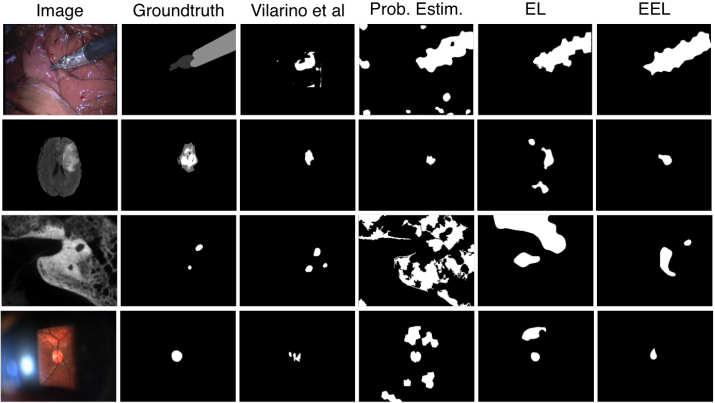
\includegraphics[width=0.99\textwidth]{qual_results}
\caption{Qualitative results. Each row shows a different dataset with an example image,
the associated desired ground truth and the produced outcome of \cite{vilarino07}, using the probability
estimation approach, EL approach and the proposed EEL.
Binary images were generated by thresholding results at a $5\%$ False Positive Rate.}
\label{fig:eel_qual_res}
\end{figure}

\subsection{Gaze variance}
In order to estimate the variance in annotations obtained with our strategy, $7$ gaze observations were performed on the same laparoscopic image sequence.
From these gaze observations, we ran our method on each set independently.
Fig. 5(left) shows the average ROC curve and standard error associated with our approach.
In addition, we show similar performances when using the EL and when using the estimated labels only.
On average we see that the EL does no better than the label estimation process, while the label estimation approach has slightly less variability.
Overall, the EEL approach not only outperforms the other settings, but has lower variance as well.

\subsection{Crowd-sourcing context}
From the 7 gaze observations collected, we consider a Crowd-Sourcing context where the label estimation is combined as described in Sec. \ref{sec:eel_estim} in order to generate the associated ground truth.
Fig. 5(right) illustrates the performance attained when doing so.
While the overall trend is no different to the previous experiment, the performance reached by the EEL approach is vastly higher.
This is unsurprising given that more gaze information is provided in this setting (i.e. 7 annotators) and that more of the object is in fact
viewed, yielding thus more positive samples, as well as better $\epsilon_{S}$ estimates.

\begin{figure}
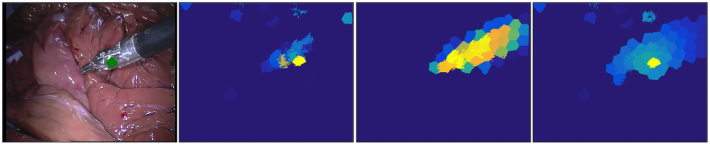
\includegraphics[width=0.99\textwidth]{propagation}
\caption{Probability propagation. Left to right: original image with the gaze location high-
lighted in green; Initial $P_{0}$ estimate from the gaze-based color model; Image regions with high
optical flow; Estimated probability after propagation. Dark blue regions depict low probability
while warmer regions correspond to higher probabilities.}
\label{fig:eel_propagation}
\end{figure}

\section{Conclusion}
In this work we have presented a strategy for domain experts to provide useful pixel-wise
annotations in a passive way. By leveraging cheap eye gaze tracking technology, we have showed
that gaze information can be used to produce segmentation ground truth in a variety of 3D
or video imaging modalities. We achieved this by introducing a novel EEL function that is
robust to large amounts of unlabeled data and few positive samples. We also demonstrated
that our approach could be used in the context of crowd-sourcing where multiple annotators
are available.
While this work presents an initial attempt, a number of aspects of this work need to
be explored moving forward. In particular, we plan to tackle the case when the object is not
present during the entire sequence, as well as cases where multiple objects are present. Naturally,
asking more of the user would provide additional information, but our goal is to keep this to a
minimum. For this reason, we also plan on determining how our method could work with noisy
object observations, as $100\%$ compliant users may not always be possible.
%%% Local Variables:
%%% mode: latex
%%% TeX-master: "../../main"
%%% End:


%----------------------------------------------------------------------------------------
%	BIBLIOGRAPHY
%----------------------------------------------------------------------------------------

\printbibliography[heading=bibintoc]

%----------------------------------------------------------------------------------------
%	BACK PAGES - Declaration of Originality
%----------------------------------------------------------------------------------------

\begin{declaration}
\addchaptertocentry{\authorshipname} % Add the declaration to the table of contents

\vspace{1cm}

\noindent {\large \bfseries Last name, first name: \authorname \par} \vspace{0.5cm}

\noindent {\large \bfseries Matriculation number: \matriculationnum \par} \vspace{2cm}

{\noindent I  hereby  declare  that  this  thesis represents my  original  work and  that  I  have  used  no  other sources except as noted by citations.\\
All  data,  tables,  figures  and  text  citations  which  have  been  reproduced  from  any  other source, including the internet, have been explicitly acknowledged as such.\\
I am aware that in case of non-compliance, the Senate is entitled to withdraw the doctorate degree awarded to me on the basis of the present thesis, in accordance with the “Statut der Universität Bern (Universitätsstatut; UniSt)”, Art. 69, of 7 June 2011.\par} \vspace{1cm}
 
 
\noindent {Place, Date:\par} \vspace{1cm}
\noindent {Signature:\par}
\end{declaration}

\end{document}  
